\subsection{Places365}\label{sec:Places365}
This in-domain dataset consists of 18 million images with 385 scene categories.
\begin{figure}[H]
    \centering
    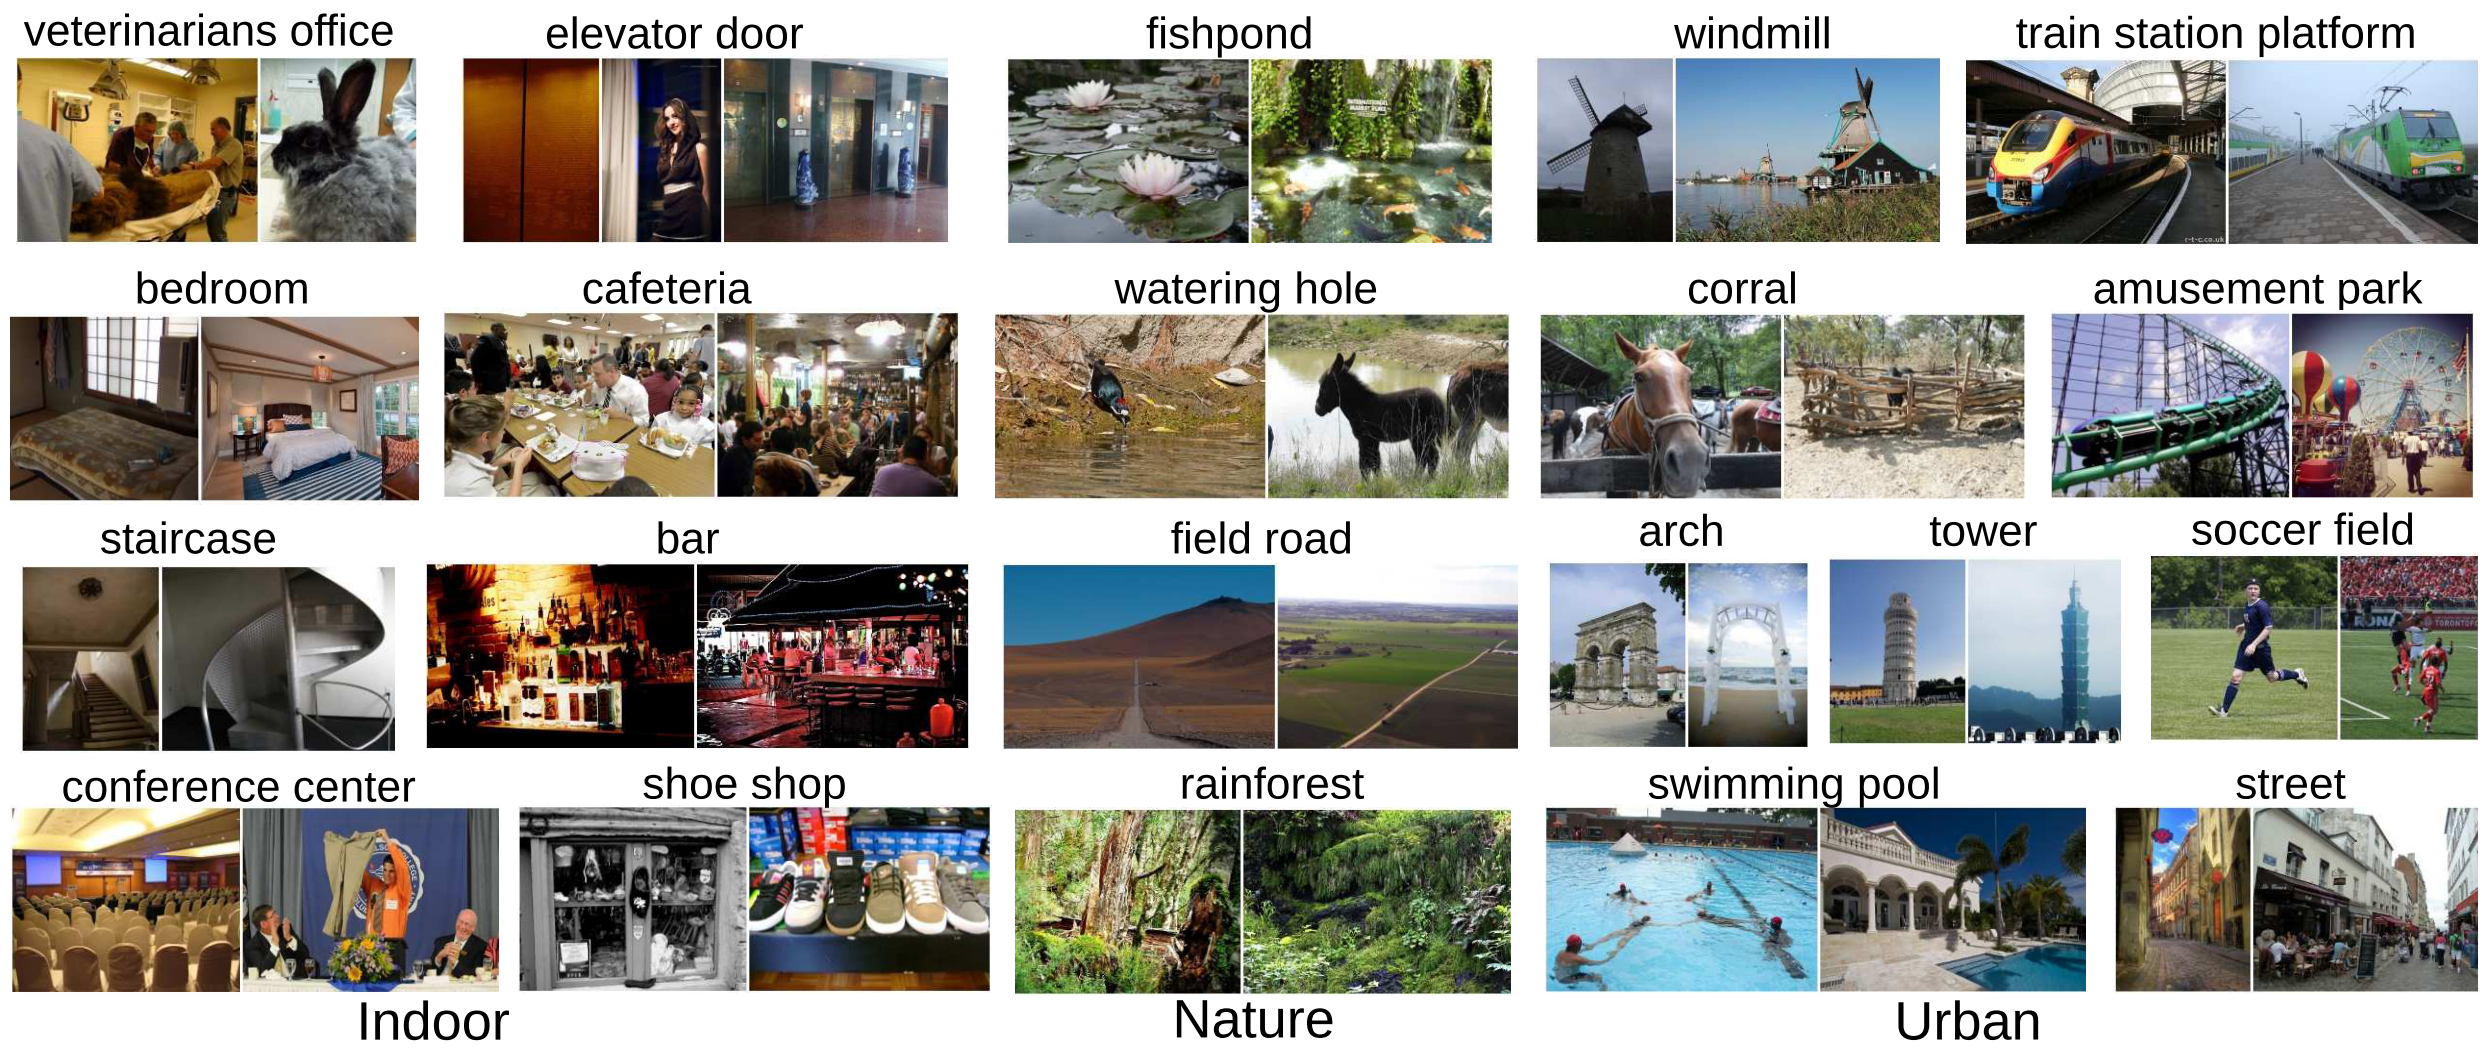
\includegraphics[scale=0.28]{pictures/random/placesart_1}
    \caption{Places macro-classes. Image source: \autocite{Places365}}
    \label{fig:placesdata1}
\end{figure}
The dataset also includes outside scenarios and objects, this might be useful if expanding the Danish Real Estate dataset to also include other classes like exterior of homes or balconies.
\begin{figure}[H]
    \centering
    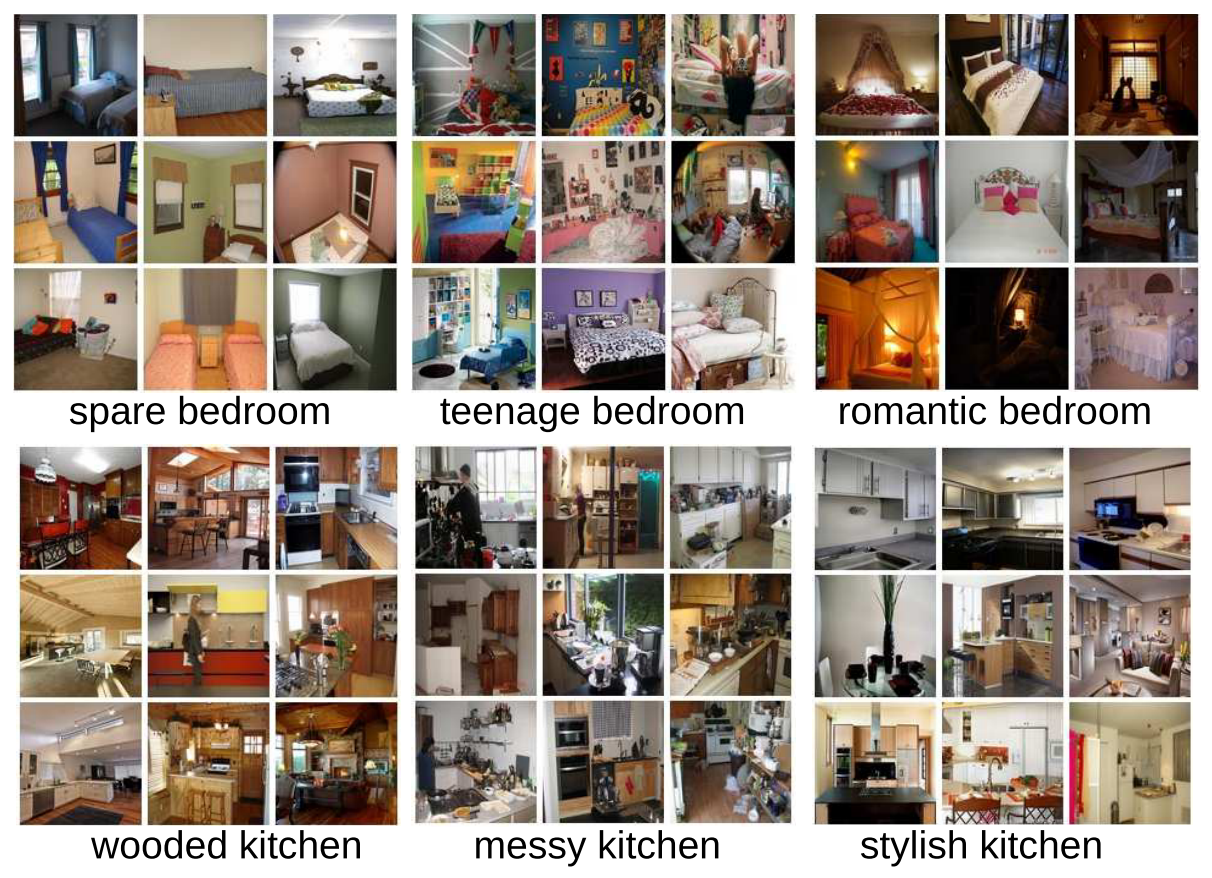
\includegraphics[scale=0.4]{pictures/random/placesart_2}
    \caption{Places indoor scene categories. Image source: \autocite{Places365}}
    \label{fig:placesdata2}
\end{figure}
The above scenarios showcase the strength that the Places365 dataset has against the ImageNet dataset. The categories of the Places365 datasets is very similar to the categories in the Danish Real Estate dataset, and it has already been proven to correctly identify similarities in \textbf{\textit{Ingwersen}}\autocite{Ingwersen}. 
